\documentclass[output=paper]{langsci/langscibook} 

\usepackage{csquotes}

\title{What can we learn from novel compounds?}

\author{Gary Libben\affiliation{Brock University}}

% \chapterDOI{} %will be filled in at production

% \epigram{}

% \abstract{Novel compounds such as \textit{shotden} and \textit{clampeel} are multiword expressions that can offer a unique perspective on the mechanisms involved in the lexical perception and production.  Because these are possible, but not existing, compound words of the language, the development of an interpretation must be based on the activation of lexical substrings as constituents. This chapter focuses on the question of how novel compounds are processed. To address this question, morphologically unambiguous compounds such as \textit{shotden} are contrasted with morphologically ambiguous compounds such as \textit{clampeel} (which can have the constituent structure \textit{clam-peel} or \textit{clamp-eel}). I discuss how these and other multimorphemic strings can be seen as \textit{lexical} \textit{superstates} and present a proposal for a simple heuristic mechanism for how they are parsed during lexical processing. This heuristic, Fuzzy Forward Lexical Activation results in binary morphological structures for a word, enables superstate representations, and thus can capture the ambiguous nature of strings such as \textit{clampeel}.  An experiment using progressive demasking to measure recognition and typing to measure production is reported.  It suggests that both versions of morphologically ambiguous strings can be activated both in recognition and production.  This provides support for the general view that all lexical substrings in a multiword expression that can be activated, will be activated.  The results are consistent with the predictions of Fuzzy Forward Lexical Activation. It is claimed that this type of activation is fundamental to the understanding of morphological effects in both the visual recognition and production of English words. Specifically, it enables the creation of \textit{morphological} \textit{superstates}, the flexible morphological structures that \citet{Libben2018} claims characterize cognitive processing in lexical comprehension and production.}

\abstract{This chapter focuses on the question of how novel compounds are processed. To address this question, morphologically unambiguous compounds such as \textit{shotden} are contrasted with morphologically ambiguous compounds such as \textit{clampeel} (which can have the constituent structure \textit{clam-peel} or \textit{clamp-eel}). I discuss how these strings can be seen as \textit{lexical superstates} and present a proposal for how they are parsed. An experiment using progressive demasking and typing is reported. Typing results show evidence of activation of both versions of ambiguous compounds,  supporting the view that all lexical substrings in a multiword expression that can be activated, will be activated.  I claim that this type of activation is fundamental to the understanding of morphological effects in both the visual recognition and production of English words. Specifically, it enables the creation of \textit{morphological superstates}, the flexible morphological structures that \citet{Libben2017} claims characterize cognitive processing in lexical comprehension and production.}

\begin{document}

\maketitle

\section{Background}\label{sec:libben:1}

\subsection{An illustrative example}\label{sec:libben:1.1}

It might be worthwhile to begin with a non-laboratory example of the type of lexical processing that needs to be accounted for.   The example begins with a furniture store in Vienna, named \textit{FantasTeak}.  To be sure, the highlighting of \textit{Teak} in the name \textit{FantasTeak} is extremely important, considering that it is a furniture store. But does the medial \textit{T} in \textit{FantasTeak} need to be capitalized?  Removing it reveals that indeed it does!  Without the medial capitalized \textit{T}, \textit{Fantasteak} seems to generate the activation of the subword \textit{steak}. Indeed, \textit{Fantasteak} is the name of a steak restaurant that opened in Campbelltown, Australia on Mother’s Day 2019. 

\textit{Fantasteak} is a highly complex and ambiguous multiword expression. It has multiple interpretations that trade on the activation of subwords such as \textit{steak}, \textit{teak} and the drink \textit{Fanta}, as well as orthographic and phonological similarity to the whole word \textit{fantastic}.  This suggests great voracity in the activation of subwords. Yet, not all subwords of the string appear to be activated. The string \textit{Fantasteak} also contains the substrings \textit{fan,} \textit{ant}, \textit{taste}, and \textit{tea}.  Although these are, on average, higher in frequency than either \textit{steak} or \textit{teak}, they seem to be relatively inaccessible within the string. The goal of this chapter is to explain why.  Why is it that some substrings of ambiguous and unambiguous compounds are activated, why other substrings are not activated, and what can this tell us about the fundamental nature of cognitive operations involved in lexical processing?

Understanding how novel morphologically complex words are parsed is key to understanding how people expand their vocabularies and indeed how morphological productivity enables new words to enter the language.  There seems to be good reason to believe that this morphological parsing and the activation of lexical substrings that it entails is not as simple and rigid as was previously thought.  As \citet{Libben2015} notes, this progression can be seen by tracing developments in the field starting with \citet{TaftForster1975}. They contrasted stimulus pairs such as \textit{replicate} and \textit{repertoire}, arguing that a word such as \textit{replicate} is perceived by native speakers of English as prefixed, whereas a word such as \textit{repertoire} is not prefixed. They predicted that, as a result, the novel prefixed form \textit{deplicat}e (containing the prefix \textit{de}{}- and an existing morphological substring \textit{-plicate}) will appear to be more word-like than the novel prefixed form \textit{depertoire} (which does not contain an existing morphological substring). Indeed, \citet{TaftForster1975} reported elevated rejection latencies for strings such as \textit{deplicate} in a lexical decision task.

The \citet{TaftForster1975} contribution was truly seminal. It was the first to invoke a process of lexical parsing and the activation of substrings to predict patterns of lexical processing across word types.  Even more importantly, from my perspective, it linked the morphological structure of a word to the manner in which it is processed by native speakers. This implies that a word such as \textit{replicate} has a prefix-stem structure because (and, perhaps, only because) people ``strip off'' the prefix during visual word processing.  

In my view, considering the morphological structure of a word in terms of what people do when they recognize or produce it, has very substantial advantages. It enables us to link the processing of novel words with the processing of existing words and it requires that we be explicit about the parsing processes that could enable the interpretation of prefixed, suffixed and compound words. Perhaps most importantly, it leads us to the view that words are actions, not things, and that morphology is what people do, not what people have. 

\subsection{Questions of lexical constituent structure}\label{sec:libben:1.2}

This leads us directly to the question: So, what is the actual morphological structure of \textit{Fantasteak}? Is it \textit{Fanta-steak}, or \textit{Fantas-steak}, or \textit{Fantas-teak}?  My answer to this question would be that the actual structure of \textit{Fantasteak} is any one of those that a language user happens to need.  Because \textit{Fantasteak} is a novel creation, it does not ``have'' any morphological structure when people first see it. Rather, it is their actions that give the word morphological structure. And, as we can see, more than one set of actions are possible. Thus, I suggest that a word such as \textit{Fantasteak} does not have a single fixed morphological structure. Rather, the characteristics of morphological processing in English create a situation in which there is both \textit{steak} and \textit{teak} in \textit{Fantasteak}. 

The formation of questions like ``Is there \textit{teak} in \textit{Fantasteak}?'' above has been at the heart of a line of psycholinguistic inquiry that has sought to isolate the conditions under which lexical substrings are and are not activated during processing. These include the \textit{hat} in \textit{that} \citep{BowersHanley2005},  the \textit{broth} in \textit{brothel} \citep{RastleNew2004}, and the \textit{corn} in \textit{corner} \citep{LongtinHalle2003,MorrisGrainger2008,LehtonenMPoeppel2011,LavricRastle2012}. For the most part, this literature has focused more on the drivers of morphological decomposition and less on the details of morphological parsing.  A key question, for example, has been whether morphological decomposition of existing words can be driven by form-based factors \citep{BeyersmannGrainger2016} or whether true morphological decomposition depends on semantic features of the word and of processing \citep{JärvikiviPyykkönen2011,RuecklAicher2008,MorrisHolcomb2007}. 

To be sure, understanding how morphological processing is influenced by formal factors and how it is influenced by the lexical semantic characteristics (e.g., the semantic transparency of the whole word) is extremely important in the development of our understanding of online lexical processing.  In this context, novel forms such as \textit{Fantasteak} may have a special role to play. The alternate morphological parses that are available for this novel string may shed light on how putative constituents are identified and the conditions under which substrings such as \textit{fantas-} can be treated by users of the language as word substrings (supported, presumably by the semantic similarity among words such as \textit{fantasia}, \textit{fantastic}, and \textit{fantasy}).

\subsection{Ambiguous novel compounds and lexical superstates}\label{sec:libben:1.3}

\citet{LibbenDerwingdeAlmeida1999} employed a type of novel morphological construction that they claimed is particularly revealing of the dynamics of morphological processing in general and morphological parsing in particular.  They focused on ambiguous novel compounds. These are novel compounds such as \textit{clampeel}, which can be parsed as either \textit{clam-peel} or \textit{clamp-eel}.  They found that there was no general tendency for native speakers of English to adopt either a first parse (e.g., \textit{clam-peel}) or last parse (e.g., \textit{clamp-eel}) approach. Moreover, they found that ambiguous novel compounds such as \textit{clampeel} show activation of all their potential constituents (e.g., \textit{clam}, \textit{clamp}, \textit{peel}, and \textit{eel}). In other words the answer to the question “Is there a (\textit{clam}, or \textit{clamp} or \textit{peel} or \textit{eel}) in \textit{clampeel}?” would simply be “Yes”.

Findings such as these call into question the assumption that a given word will have a univocal morphological structure.  \citet{Libbeninpress} argues that this indeterminacy applies to the morphology of lexical structures in general.  Under this view, a string such as \textit{clampeel} can be described as being in a lexical superstate – a cognitive state that is best described by the opportunities for interpretation that it enables.  \citet{Libbeninpress} claims that this applies to morphological structures in general. Thus, an existing compound such as \textit{keyboard} has, as a superstate, the whole word representation \textit{keyboard} as well as the decomposed representation \textit{key-board}. Analogously, an existing suffixed word such as \textit{formality} can be best described as having the lexical superstate representation shown in \figref{fig:libben:1}. In this figure, the string has a whole word representation as well as multiple decomposition possibilities. Which one of these is actually implemented in an act of lexical processing will depend on the specifics of the processing task, the individual language user, and the situation in which they are found.


\begin{figure}
%%please move the includegraphics inside the {figure} environment
%%\includegraphics[width=\textwidth]{figures/PMW18paperLibben-img001.emf}
    \begin{tikzpicture}[rotate=45,transform shape]
    \draw [draw,fill=lsLightGray,even odd rule,name=nucleus]  (0,0) circle (3mm)  (0,0) circle (.5mm);
    \coordinate (nucleus) at (0,0);
    \node [right=3mm of nucleus.east] {[formal][ity]};
    \node [left=3mm of nucleus.west,anchor=east] {[form][al][ity]};
    \node [below=3mm of nucleus.south,rotate=-90,anchor=west] {[formality]};
    \node [above=3mm of nucleus.north,rotate=-90,anchor=east] {[form][ality]};
    \end{tikzpicture}
\caption{\label{fig:libben:1}An example lexical superstate representation. The word \textit{formality} can be undecomposed, fully decomposed, have a suffix string (\textit{-ality}) or a complex stem (\textit{formal}).}
\end{figure}

Lexical superstate representations can also be effective in capturing the structural ambiguity of a word such as \textit{unlockable} in \figref{fig:libben:2}, which can be interpreted as `not lockable' (\textit{un-lockable}) or `able to be unlocked' (\textit{unlock-able}). Lexical superstate representation can also be applied to novel ambiguous strings such as \textit{Fantasteak} and \textit{clampeel}. These are shown in \figref{fig:libben:3}. As can be seen in this figure, in many ways, the novel string \textit{Fantasteak} is the more complex of the two. In order to capture the key features of \textit{Fantasteak}, it is necessary to indicate that it is linked in an unspecified manner (represented by a dotted line) to the existing word \textit{fantastic} (and \textit{fantasy}, etc.). This acknowledges the likely source of both novel interpretations. It also leads to the requirement to accept a fuzzy parse such as \textit{Fantas-steak}, in which the medial \textit{s} is repeated.\largerpage[-1]


\begin{figure}
    \begin{tikzpicture}[rotate=45,transform shape]
    \draw [draw,fill=lsLightGray,even odd rule,name=nucleus]  (0,0) circle (3mm)  (0,0) circle (.5mm);
    \coordinate (nucleus) at (0,0);
    \node [right=3mm of nucleus.east] {[unlock][able]};
    \node [left=3mm of nucleus.west,anchor=east] {[un][lock][able]};
    \node [below=3mm of nucleus.south,rotate=-90,anchor=west] {[unlockable]};
    \node [above=3mm of nucleus.north,rotate=-90,anchor=east] {[un][lockable]};
    \end{tikzpicture}
\caption{\label{fig:libben:2}Superstate representations for the structurally ambiguous word \textit{unlockable}.}
\end{figure}

\begin{figure} 
    \centering
    \begin{minipage}{.5\linewidth}%
    \begin{tikzpicture}
    \draw [draw,fill=lsLightGray,even odd rule,name=nucleus]  (0,0) circle (3mm)  (0,0) circle (.5mm);
    \coordinate (nucleus) at (0,0);
    \node [above right= .5\baselineskip and 3mm of nucleus.north east,anchor=west,rotate=45] {[Fanta][steak]};
    \node [above left= .5\baselineskip and 3mm of nucleus.north west,anchor=east,rotate=-45] {[Fantas][teak]};
    \node [below=3mm of nucleus.south,rotate=-90,anchor=west] {[Fantas][steak]};
    \node (fantastic) [above=3\baselineskip of nucleus.north] {\itshape fantastic};
    \draw[dotted,thick] (fantastic) -- (nucleus.north) +(0,-3mm);
    \end{tikzpicture}\end{minipage}\begin{minipage}{.5\linewidth}%
    \begin{tikzpicture}
    \draw [draw,fill=lsLightGray,even odd rule,name=nucleus]  (0,0) circle (3mm)  (0,0) circle (.5mm);
    \coordinate (nucleus) at (0,0);
    \node [above right= .5\baselineskip and 3mm of nucleus.north east,anchor=west,rotate=45] {[clamp][eel]};
    \node [above left= .5\baselineskip and 3mm of nucleus.north west,anchor=east,rotate=-45] {[clam][peel]};
    \node [below=3mm of nucleus.south,rotate=-90,anchor=west] {[clamp][peel]};
    \end{tikzpicture}\end{minipage}
\caption{\label{fig:libben:3}Superstate representations for novel compounds. \textit{Fantasteak} is shown on the left.  The dotted line indicates an association to the existing word \textit{fantastic}.  \textit{Clampeel} is shown on the right.}
\end{figure}

The representation\largerpage[-1] of \textit{clampeel} in \figref{fig:libben:3} has a structure that has features in common with that of \textit{Fantasteak}.  It shows the possibility of a fuzzy parse in which the medial letter is repeated (in this case the medial \textit{p} to enable the interpretation \textit{clamp-peel}).  Overall, however, \textit{clampeel} is quite a bit more controlled and straightforward than \textit{Fantasteak}. First, we can be relatively confident that \textit{clam} and \textit{clamp} are existing lexical strings of English. This is not necessarily the case for \textit{Fanta} (the name of a drink produced by Coca Cola) or \textit{fantas} (which may or may not be a unit of recognition for speakers of English). Second, the interpretation cannot draw on the interpretation of a set of existing words (as is the case for Fantasteak).  Ambiguous novel compounds such as \textit{clampeel}, therefore, may constitute the stimulus type that would enable us to investigate the \textit{Fantasteak} phenomenon under relatively controlled conditions. In addition, ambiguous novel compounds provide a testing ground for the investigation of how readers of English are able to make use of the advantages enabled by compound word productivity in the context of a writing system in which compound words are often written as single unspaced strings. 

\subsection{Fuzzy Forward Lexical Activation generates lexical superstate representations}\label{sec:libben:1.4}

Why are English language users likely to find \textit{clam} and \textit{clamp} in \textit{clampeel}? And why are they less likely to find the substrings \textit{lamp}, \textit{am}, and \textit{amp}? \citet{TaftForster1976} claimed that, fundamentally, morphological processing was a left-to-right process in the reading of English.  

There is a good deal of evidence that supports the assumption that morphological activation is achieved through beginning-to-end processing. However, it is less clear that morphemes themselves have discreet representations in the mental lexicon (e.g., \citealt{BaayenSmolka2019,RamscarEtAl2018}).  In addition, phenomena such as the shared \textit{s} in \textit{Fantas-steak} suggest that an approach to parsing that requires that reference be made to fixed individual morphemes and individual letters in a word is likely to be problematic.  A more useful approach to capturing how individuals identify constituent substrings of English words can be to simply posit a heuristic of Fuzzy Forward Lexical Activation. In this approach, processing always takes place from beginning to end. Initial letters of a word are scanned until a familiar initial lexical substring is encountered. If it is, a final substring is computed from that position onward. If that final substring is also familiar, it is interpreted and the process continues.  Thus, the strings \textit{formality}, \textit{clampeel}, \textit{Fantasteak}, and \textit{unlockable} would be processed in the manner shown in \tabref{tab:libben:1}.

\begin{table}
\caption{\label{tab:libben:1}Fuzzy Forward Lexical Activation for stimuli such as \textit{formality,} \textit{clampeel,} \textit{Fantsteak}, and \textit{unlockable}.}
\begin{tabular}{c*{4}{>{\itshape}l}}
\lsptoprule

{Parse}  & \multicolumn{4}{c}{{Stimuli}}\\\cmidrule(lr){2-5}
& \textit{formality} & \textit{clampeel} & \textit{Fantastic} & \textit{unlockable}\\\midrule
 1. & form-ality & clam-peel & Fanta-steak & un-lockable\\
 2. & formal-ity & clamp-eel & Fantas-teak & unlock-able\\
 3. & formality & (+clamp-peel) & (+Fantas-steak) & unlockable\\
\lspbottomrule
\end{tabular}
\end{table}

This parsing heuristic makes the claim that processing activity will generate patterns that correspond to both readings of a novel ambiguous word such as \textit{clampeel}, as well as an existing structurally ambiguous word such as \textit{unlockable}, simply by parsing them.

In addition, the parsing heuristic will generate both stem-suffix representations for the word \textit{formality}, as well as an affix string representation. It will, however, neither generate the fully decomposed representation \textit{form-al-ity} nor the fully decomposed representation \textit{un-lock-able.} The heuristic therefore makes the empirical claim that English language users do not create such fully decomposed representations either.  They are thus claimed to be potential lexical superstate representations that are not realized because of the dynamics of visual lexical processing in English.

%\subsubsection{Looking right creates binary structures}\label{sec:libben:1.4.1}

Fuzzy Forward Lexical Activation is likely the simplest possible approach to English visual morphological parsing. Like the signs that one sees on London crosswalks to aid tourists, it says: “Look right →”.  By beginning at the beginning and looking right it ensures that the key initializing activity in morphological processing is the activation of the initial substring of the word. Thus, although this approach to morphological processing differs from the prefix-stripping approach of \citet{TaftForster1975}, it has much the same effect.  The processing of a word such as \textit{unlockable} begins with the recognition of the prefix \textit{un-}. 
From there, the parses \textit{un-lockable}, \textit{unlock-able} are created (under the assumption that the substrings \textit{lockable}, \textit{unlock} and \textit{-able} are known to the language user). This feature of checking that substring to the right is known to the language user ensures that the parse \textit{form-ality} is possible under the assumption that a language user maintains a trace of suffix strings such as \textit{-ality} \citep{Derwing2014,LibbenJaremaEtAl2016}.  However, the potential parse \textit{for-mality} would fail at the “look right” stage because the string \textit{-mality} is unlikely to be known to the language user as a representation of English.


% % % % From there, the parses \textit{un-lockable}, \textit{unlock-able} are created (under the assumption that the substrings \textit{lockable}, \textit{unlock} and \textit{{}-able} are known to the language user).

Fuzzy Forward Lexical Activation constituted an extremely simple approach to morphological parsing that, I claim, is linked directly to the lexical superstate representations shown in Figures~\ref{fig:libben:1}, \ref{fig:libben:2} and~\ref{fig:libben:3}. Indeed, it creates them.  Its functioning results in morphological processing that is primarily binary. The reason for this is that it must begin at the beginning and it must look toward the end of the word. The functioning of Fuzzy Forward Lexical Activation also results in what might be termed hierarchical morphological structure, so that a word such as \textit{undrinkable} would be parsed as the right-branching structure \textit{un-drinkable,} whereas a word such as \textit{unlockable} will be parsed as both the right-branching structure \textit{un-lockable} and the left-branching structure \textit{unlock-able}.

\subsection{Typing as a window to morphological processing}\label{sec:libben:1.5}

This brings us to the question how the predictions of the lexical superstate hypothesis and the proposed mechanisms of Fuzzy Forward Lexical Activation can be evaluated.  A potentially revealing task is one that specifically targets lexical activation in left-to-right processing.  I suggest that the online typing of words is exactly such a task.  In online typing, a participant is presented with a lexical string and is asked to type it as quickly and as accurately as possible.  For each word typed, it is possible to calculate overall per letter typing times as well as per letter typing times at specific locations in the word \citep{FeldmanEtAl2019,LibbenJaremaEtAl2016,SahelWeingarten2008,WillWeingarten2006}.

If indeed, morphological structure for novel compounds is evident in online typing, we should see elevated response times at the morpheme boundary for unambiguous strings such as \textit{anklecob.} This would correspond to the location at which participants recognize an initial string \textit{ankle} and then would look right to the end of the string, recognizing \textit{cob}. For ambiguous novel compounds such as \textit{clampeel}, however, the location of the putative morpheme boundary should be blurred and both potential parses should become part of the lexical superstate.  We would expect elevated letter typing times at both the locations between \textit{clam} and \textit{peel}, as well as between \textit{clamp} and \textit{eel}.  %%%These predictions were investigated in the experiment reported below.
Our previous research has shown that the typing of morphologically complex words is characterized by elevated typing times at the constituent boundary \citep{LibbenWeber2014,LibbenJaremaEtAl2016}. This difference in typing time may reflect morphological chunking in letter typing, so that a two constituent compound word is typed as a sequence of two motor plans. Each motor plan would correspond to a compound constituent. The prediction regarding typing times for ambiguous novel compounds follows from this observation: If the production of ambiguous novel compounds involves the activation of all potential constituents, then we should expect that four motor plans are in play.  This would result in ``blurring'', i.e., longer and lower latency spikes. Latency increases would be longer because they would be spread over two letter boundaries rather than one and they would be lower because each of those letter boundaries is at once a ``between constituent'' location and a ``within-constituent'' location.

Thinking about constituent boundary effects in terms of motor plans suggests that a number of control variables also need to be tracked.  The reason for this is that one would expect that the speed with which word typing motor plans are created and executed can be influenced by position in the word and by the frequency of particular letter combinations in the language. Moreover, particular attention would need to be paid to letter co-occurrence frequencies at the constituent boundary itself.  These predictions and analytic considerations were tested in the experiment described below.

\section{Method}\label{sec:libben:2}

\subsection{Participants}\label{sec:libben:2.1}

Twenty-four native English speakers between the age of 17 and 26 years participated in the study.  All reported English to be their mother tongue and none had learned a second language before age ten.  All participants had normal or corrected-to-normal vision. They were all university students from a variety of departments of Brock University who received either course credit or \$15 for their participation.

\subsection{Stimuli}\label{sec:libben:2.2}
In total, participants viewed and produced 45 stimuli, all of which were novel  noun-noun English compounds. Fifteen of these were unambiguous novel compounds, thirty were ambiguous novel compounds. The ambiguous novel compound stimuli were created by extracting all nouns from the CELEX database \citep{BaayenGulikers1995} and then identifying which of those also created nouns when their last letter was removed. This created a candidate first constituent pair (e.g. \textit{clam}, \textit{clamp}). Each such pair was then linked to a noun in the CELEX database that began with the last letter of the longer member of the pair (in this case, \textit{p}) and which also created a noun when its first letter is removed (e.g., \textit{peel}, \textit{eel}). This process of selection creates the set of English novel noun-noun compound stimuli such as \textit{clampeel}.  The resulting set of 45 stimuli are shown in \tabref{tab:libben:2}.  These were created so that constituents were comparable in frequency and length. The set of ambiguous novel compounds was subdivided into those in which the grapheme-to-phoneme relations were different in each of the two parses and those for which the grapheme-to-phoneme relations were essentially the same. The difference between these two subgroups can be easily appreciated by reading aloud the stimuli in the middle column of \tabref{tab:libben:2} and reading aloud those in the final column of the table. The ambiguous stimuli with sound change shown in the middle column are those such as \textit{babelarch}. As \textit{babe-larch}, the first constituent is one syllable in length and has the initial vowel /ej/. As \textit{babel-arch}, the first constituent is two syllables in length and has the initial vowel /æ/.  In contrast, \textit{clampeel}, as the first stimulus in the third column of \tabref{tab:libben:2}, has essentially the same phonological realization as \textit{clam-peel} and \textit{clamp-eel} (assuming co-articulation and other effects associated with the morpheme boundary).

\begin{table}
\caption{\label{tab:libben:2}The novel compound stimuli in the progressive demasking and typing tasks.  Unambiguous stimuli (e.g., \textit{anklecob}) have a single morphological parse (e.g., \textit{ankle}\,+\,\textit{cob}). Ambiguous stimuli (e.g., \textit{clampeel,} \textit{babelarch)} have two possible morphological parses. For the ones with sound change, the pronunciation of graphemes depends on the parse (e.g., \textit{babe}\,+\,\textit{larch}, \textit{babel}\,+\,\textit{arch}).  For ambiguous stimuli without sound change, it does not (e.g., \textit{clam}\,+\,\textit{peel}, \textit{clamp}\,+\,\textit{eel}).}
\begin{tabular}{*{3}{>{\itshape}l}}
\lsptoprule
{\normalfont Unambiguous} & \multicolumn{2}{c}{{\normalfont Ambiguous}}\\\cmidrule(lr){2-3}
& {\normalfont with sound change} & {\normalfont without sound change}\\\midrule
anklecob & babelarch & clampeel\\
clubswim & bandanger & crampinch\\
deckswerve & bowlease & damplane\\
fakebread & cardevil & fangape\\
floataxe & cellorange & feedraft\\
friendbotany & dudemission & firmaid\\
kelpfibre & fatemotion & fundrain\\
lyricalp & findrag & rumplight\\
plazafocus & grindream & rungear\\
shotden & gripequality & scarfright\\
spillcarriage & kindrift & sealedge\\
squeakpub & modelore & songlass\\
supplychase & realmink & spamoral\\
watchpanic & sodacorn & teamother\\
whiffpalace & winglint & wardrug\\
\lspbottomrule
\end{tabular}
\end{table}

% \subsection{Apparatus and procedure}\label{sec:libben:2.3}
% The procedure employed in the present study was implemented in Psyscope X, running on a MacBook Pro, using an IO Labs button box Voice Key.  
% 
% We used a combined progressive demasking and typing paradigm as developed by \citet{LibbenEtAl2012} and \citet{LibbenWeber2014}. In this paradigm, participants first see a word being progressively demasked in the center of a computer screen. and must identify it as quickly as possible. After the word is identified (either by saying it aloud or by pressing the return key), the stimulus disappears. The participant is then asked to type it as quickly and as accurately as possible. 
% 
% \todo[inline]{Please insert more details: e.g. Each participant saw all 45 words; randomization?}
% 
% \subsubsection{Progressive demasking}\label{sec:libben:2.3.1}
% 
% The key feature of the progressive demasking is that words appear very slowly as though they were emerging from a fog.  This effect was created in this experiment by alternating the presentation of a stimulus word and a pattern mask of cross hatches (\#\#\#\#\#\#\#\#\#\#) over 18 cycles. Each cycle was 300\,ms in length.  In the first cycle, the target word is presented for only 16\,ms and the mask is presented for 284\,ms. In the next cycle, the target is presented for 16\,ms longer than in the previous cycle and the mask is presented for 16\,ms less (i.e., 32\,ms and 268\,ms respectively), Thus, in each successive cycle, the target word becomes more visible.  Typically, for real and novel compound words, the stimulus word is identified in under 10 cycles (3,000\,ms). In the present study, participants were randomly assigned to one of two progressive demasking procedures. The difference between the groups was that Group 1 participants were asked to press the keyboard return key as soon as they could identify the word. Group 2 participants were asked to say the word aloud as soon as they could identify it.
% 
% \subsubsection{Typing}\label{sec:libben:2.3.2}
% 
% For each stimulus, the typing component of the task began immediately following the participant’s identification of the progressively demasked stimulus.  Typing was done on a standard laptop keyboard, and the letters that the participant typed were visible on the screen (as is the case in normal typing).  Participants were able to self-correct during word typing by pressing the backspace key. As soon as they finished typing the word, they pressed the return key. This initiated the next trial.

\section{Apparatus and procedure}\label{sec:libben:2.3}
The procedure employed in the present study was implemented in Psyscope X, running on a MacBook Pro, using an IO Labs button box Voice Key. 

We used a combined progressive demasking and typing paradigm as developed by \citet{LibbenEtAl2012} and \citet{LibbenWeber2014}. In this paradigm, participants first see a word being progressively demasked in the center of a computer screen. and must identify it as quickly as possible. After the word is identified (either by saying it aloud or by pressing the return key), the stimulus disappears. The participant is then asked to type it as quickly and as accurately as possible. 

All 24 participants identified and typed all 45 stimulus words. Stimuli were presented in a different random order for each participant.  Testing was conducted in a single block of trial and the main experiment was preceded by a practice session of six trails.

Each trial consisted of two components:  a progressive demasking component and a typing component, with an inter-trial interval of two seconds.  Thus, in the first trial of the experiment, a participant would see word being progressively demasked and would identify it. This progressive demasking component would be immediately followed by the typing component. The screen would go blank and the participant would type the word using the keyboard of the MacBook Pro. Participants pressed the return key after they had typed the last letter of the stimulus word. That action initiated the appearance of the target stimulus in the center of the string. Participants were asked to verify that this was in fact the stimulus that they saw by pressing a key marked “yes” or “no” on the keyboard (all participants responded “yes” to all words).  Their pressing of the “yes” key ended the trial. The screen then went blank for 2 seconds, after with the progressive demasking component of the next trial began.  The details of each of two the trial components are presented below.

\subsection{The progressive demasking component}\label{sec:libben:2.3.1}
The key feature of the progressive demasking is that words appear very slowly as though they were emerging from a fog. This effect was created in this experiment by alternating the presentation of a stimulus word and a pattern mask of cross hatches (\#\#\#\#\#\#\#\#\#\#) over 18 cycles. Each cycle was 300\,ms in length. In the first cycle, the target word is presented for only 16\,ms and the mask is presented for 284\,ms. In the next cycle, the target is presented for 16\,ms longer than in the previous cycle and the mask is presented for 16\,ms less (i.e., 32\,ms and 268\,ms respectively), Thus, in each successive cycle, the target word becomes more visible. Typically, for real and novel compound words, the stimulus word is identified in under 10 cycles (3,000\,ms). In the present study, participants were randomly assigned to one of two progressive demasking procedures. The difference between the groups was that Group 1 participants were asked to press the keyboard return key as soon as they could identify the word. Group 2 participants were asked to say the word aloud as soon as they could identify it. These two groups were created in order to test whether saying the stimuli aloud in the progressive demasking task would have the effect of disambiguating the ambiguous stimuli in the subsequent typing task.

\subsection{The typing component}\label{sec:libben:2.3.2}
For each stimulus, the typing component of the task began immediately following the participant’s identification of the progressively demasked stimulus. Typing was done on a standard laptop keyboard, and the letters that the participant typed were visible on the screen (as is the case in normal typing). Participants were able to self-correct during word typing by pressing the backspace key. As soon as they finished typing the word, they pressed the return key. This ended the typing component of the trial.

\section{Results}\label{sec:libben:3}

Our analysis focused on trials in which stimuli were typed without error (i.e., the word produced was that which was presented and was typed without the backspace key having been pressed).  The overall accuracy rate, defined in this way, was 79\%. The progressive demasking response latencies and letter typing times for correctly typed stimuli were analyzed using linear mixed effects models in R.

\subsection{Progressive demasking}\label{sec:libben:3.1}\largerpage

The analysis of progressive demasking latencies in a generalized linear mixed effects model did not yield significant effects of recognition latency differences related to whether the stimulus was ambiguous, whether the ambiguity resulted in a pronunciation change, or whether participants responded by saying the word aloud or by pressing the return key. There was, however, a facilitating effect of the frequency of the initial substring of the stimulus ($p<0.001$). This is consistent with the expectation that Fuzzy Forward Lexical Activation is driven by the familiarity of an initial lexical substring. No other significant lexical frequency effects were observed in the progressive demasking task or in the typing task (e.g., for a stimulus such as \textit{clampeel}, the frequency of \textit{clam} had an effect, but the frequencies of \textit{clamp}, \textit{peel}, or \textit{eel} did not). Lexical frequency values were obtained from the CELEX English lemma databases \citep{BaayenGulikers1995}.


\subsection{Typing}\label{sec:libben:3.2}
In the analysis of typing times, the random effects included participant, stimulus and letter typed. This last random effect was included to capture the influences of factors that could be associated with the typing of a particular letter on a keyboard. These may include whether it is a consonant or a vowel, whether it is typed with the right hand or left hand, the index finger or some other finger, etc.

The two key fixed effects in the model were the position of the letter with respect to the constituent boundary and stimulus ambiguity (ambiguous vs.\ nonambiguous). For the variable ``letter location around boundary'', four locations were targeted: 

\begin{enumerate}
\item the letter before the first constituent boundary (e.g., \textit{m} in \textit{clampeel}). This is on the intercept; 
\item the letter at the first constituent boundary (e.g., \textit{p} in \textit{clampeel});
\item the letter at the second constituent boundary (e.g., the first \textit{e} in \textit{clampeel});
\item the letter after the second constituent boundary (e.g., the second \textit{e} in \textit{clampeel});
\end{enumerate}\largerpage[2]

This factor was investigated as a fixed effect and in terms of its interaction with stimulus ambiguity. 

There was no effect or interaction associated with whether the participant responded in the progressive demasking task by pressing the return key or by saying the stimulus aloud ($p>0.1$). This variable was removed from the model and the participants were treated as a single group.

The analysis began with the two key factors above. To this, a number of control factors were added. These included trial ($p=0.003$), which indicated that participants' typing got faster as they progressed through the experiment. The variable ``position within the word'' was also added. This variable, which was marginally significant ($p=0.049$), showed a tendency for participants to be somewhat slower at later points in the word. The inclusion of this factor improved the model and acted as a control for the fact that the first constituent boundary for some stimuli (e.g., \textit{clampeel}) was at letter 5 of the stimulus, whereas, for others, (e.g., \textit{damplane}) it was at letter 4. Stimuli with constituent boundaries later in the string were associated with slower typing times.

The four additional control variables that were added to the model all concern the frequency of letter sequences. All improved model performance. The first was the overall bigram frequency of the stimulus string, obtained from the English Lexicon Project \citep{BalotaEtAl2007}. The second was the frequency of the letter being typed in combination with its preceding letter. The third was the frequency of the letter being typed in combination with its following letter. Finally, the fourth variable was the frequency of the two-letter sequence at the first constituent boundary. Whereas, in the first three bigram frequency measures, higher frequency was associated with faster typing times, the opposite was the case for bigram frequency at the constituent boundary. Here, higher bigram frequency slowed typing times. This observation is consistent with the view that typing involves chunking by constituent and therefore, high frequency bigram transitions that could potentially disrupt the segmentation of the novel compound into constituents are disruptive.

The results of typing times showed effects of bigram frequency, location with respect to constituent boundaries, and ambiguity.  The analysis of these data patterns is presented in \tabref{tab:libben:5} and \figref{fig:libben:4}.\largerpage

As can be seen in \figref{fig:libben:4}, the non-ambiguous stimuli (e.g., \textit{anklecob}) show a clear typing pause at the constituent boundary. That is, at the point at which they type the first letter of the second constituent (e.g., the \textit{c} in \textit{anklecob}). Letter typing times for the following letter drop considerably to below 200 milliseconds immediately following that letter. In contrast, that same position shows typing times in the 250 millisecond range for ambiguous stimuli. The key difference is that, for ambiguous stimuli, that position (e.g., the \textit{e} in \textit{clampeel}), is at once a constituent boundary in the reading \textit{clamp-eel} and the second letter in the reading \textit{clam-peel}. This dual status seems to be reflected in the per letter typing times shown in \figref{fig:libben:4}. 

\begin{sidewaystable}
\caption{Fixed effects of the predictors in the linear mixed effects model for letter typing times. (Note: \text{*} = $p < 0.05$; \text{**} = $p < 0.01$; $\text{***} = p < 0.001$)\label{tab:libben:5}}
\begin{tabular}{clSSSSS[table-format=<1.3]l}
\lsptoprule
 ID & Factor and level names &  {Estimate} &  {Std. Error} &  {df} &  {\textit{t}-value} &  {$p$} & \\\midrule
 1 & (Intercept) &  618.8 &  131.3 &  61.5 &  4.7 &  >.001 & ***\\
 2 & Bigram Freq. &  -27.6 &  15.0 &  40.0 &  -1.8 &  .073 & \\
 3 & Trial &  -0.5 &  0.2 &  3246.6 &  -3.0 &  .003 & **\\
 4 & Position in word &  17.8 &  8.7 &  39.4 &  2.0 &  .049 & *\\
 5 & Freq. of letter and its predecessor &  -22.8 &  3.5 &  1083.6 &  -6.5 &  .000 & ***\\
 6 & Freq. of letter and its successor &  -8.4 &  3.1 &  1474.2 &  -2.7 &  .008 & **\\
 7 & Freq. of bigram at boundary 1 &  16.3 &  4.9 &  40.9 &  3.3 &  .002 & **\\
 8 & Letter is 2nd constituent onset (v.1) &  30.9 &  13.1 &  189.3 &  2.4 &  .019 & *\\
 9 & Letter is 2nd constituent onset (v.2) &  43.1 &  19.8 &  64.8 &  2.2 &  .033 & *\\
 10 & Letter is 2nd constituent letter 3 (v.1) &  -31.8 &  27.6 &  48.7 &  -1.2 &  .255 & \\
 11 & Nonambiguous stimulus &  5.3 &  20.9 &  69.1 &  0.3 &  .801 & \\
 12 & Interaction of 8 X 11 &  59.2 &  17.2 &  2288.3 &  3.4 &  .001 & ***\\
 13 & Interaction of 9 X  11 &  -80.3 &  17.1 &  1937.3 &  -4.7 &  .000 & ***\\
 14 & Interaction of 10 X  11 &  -17.5 &  18.2 &  2599.8 &  -1.0 &  .338 & \\
\lspbottomrule
\end{tabular}
\end{sidewaystable}
  
  
\begin{figure}
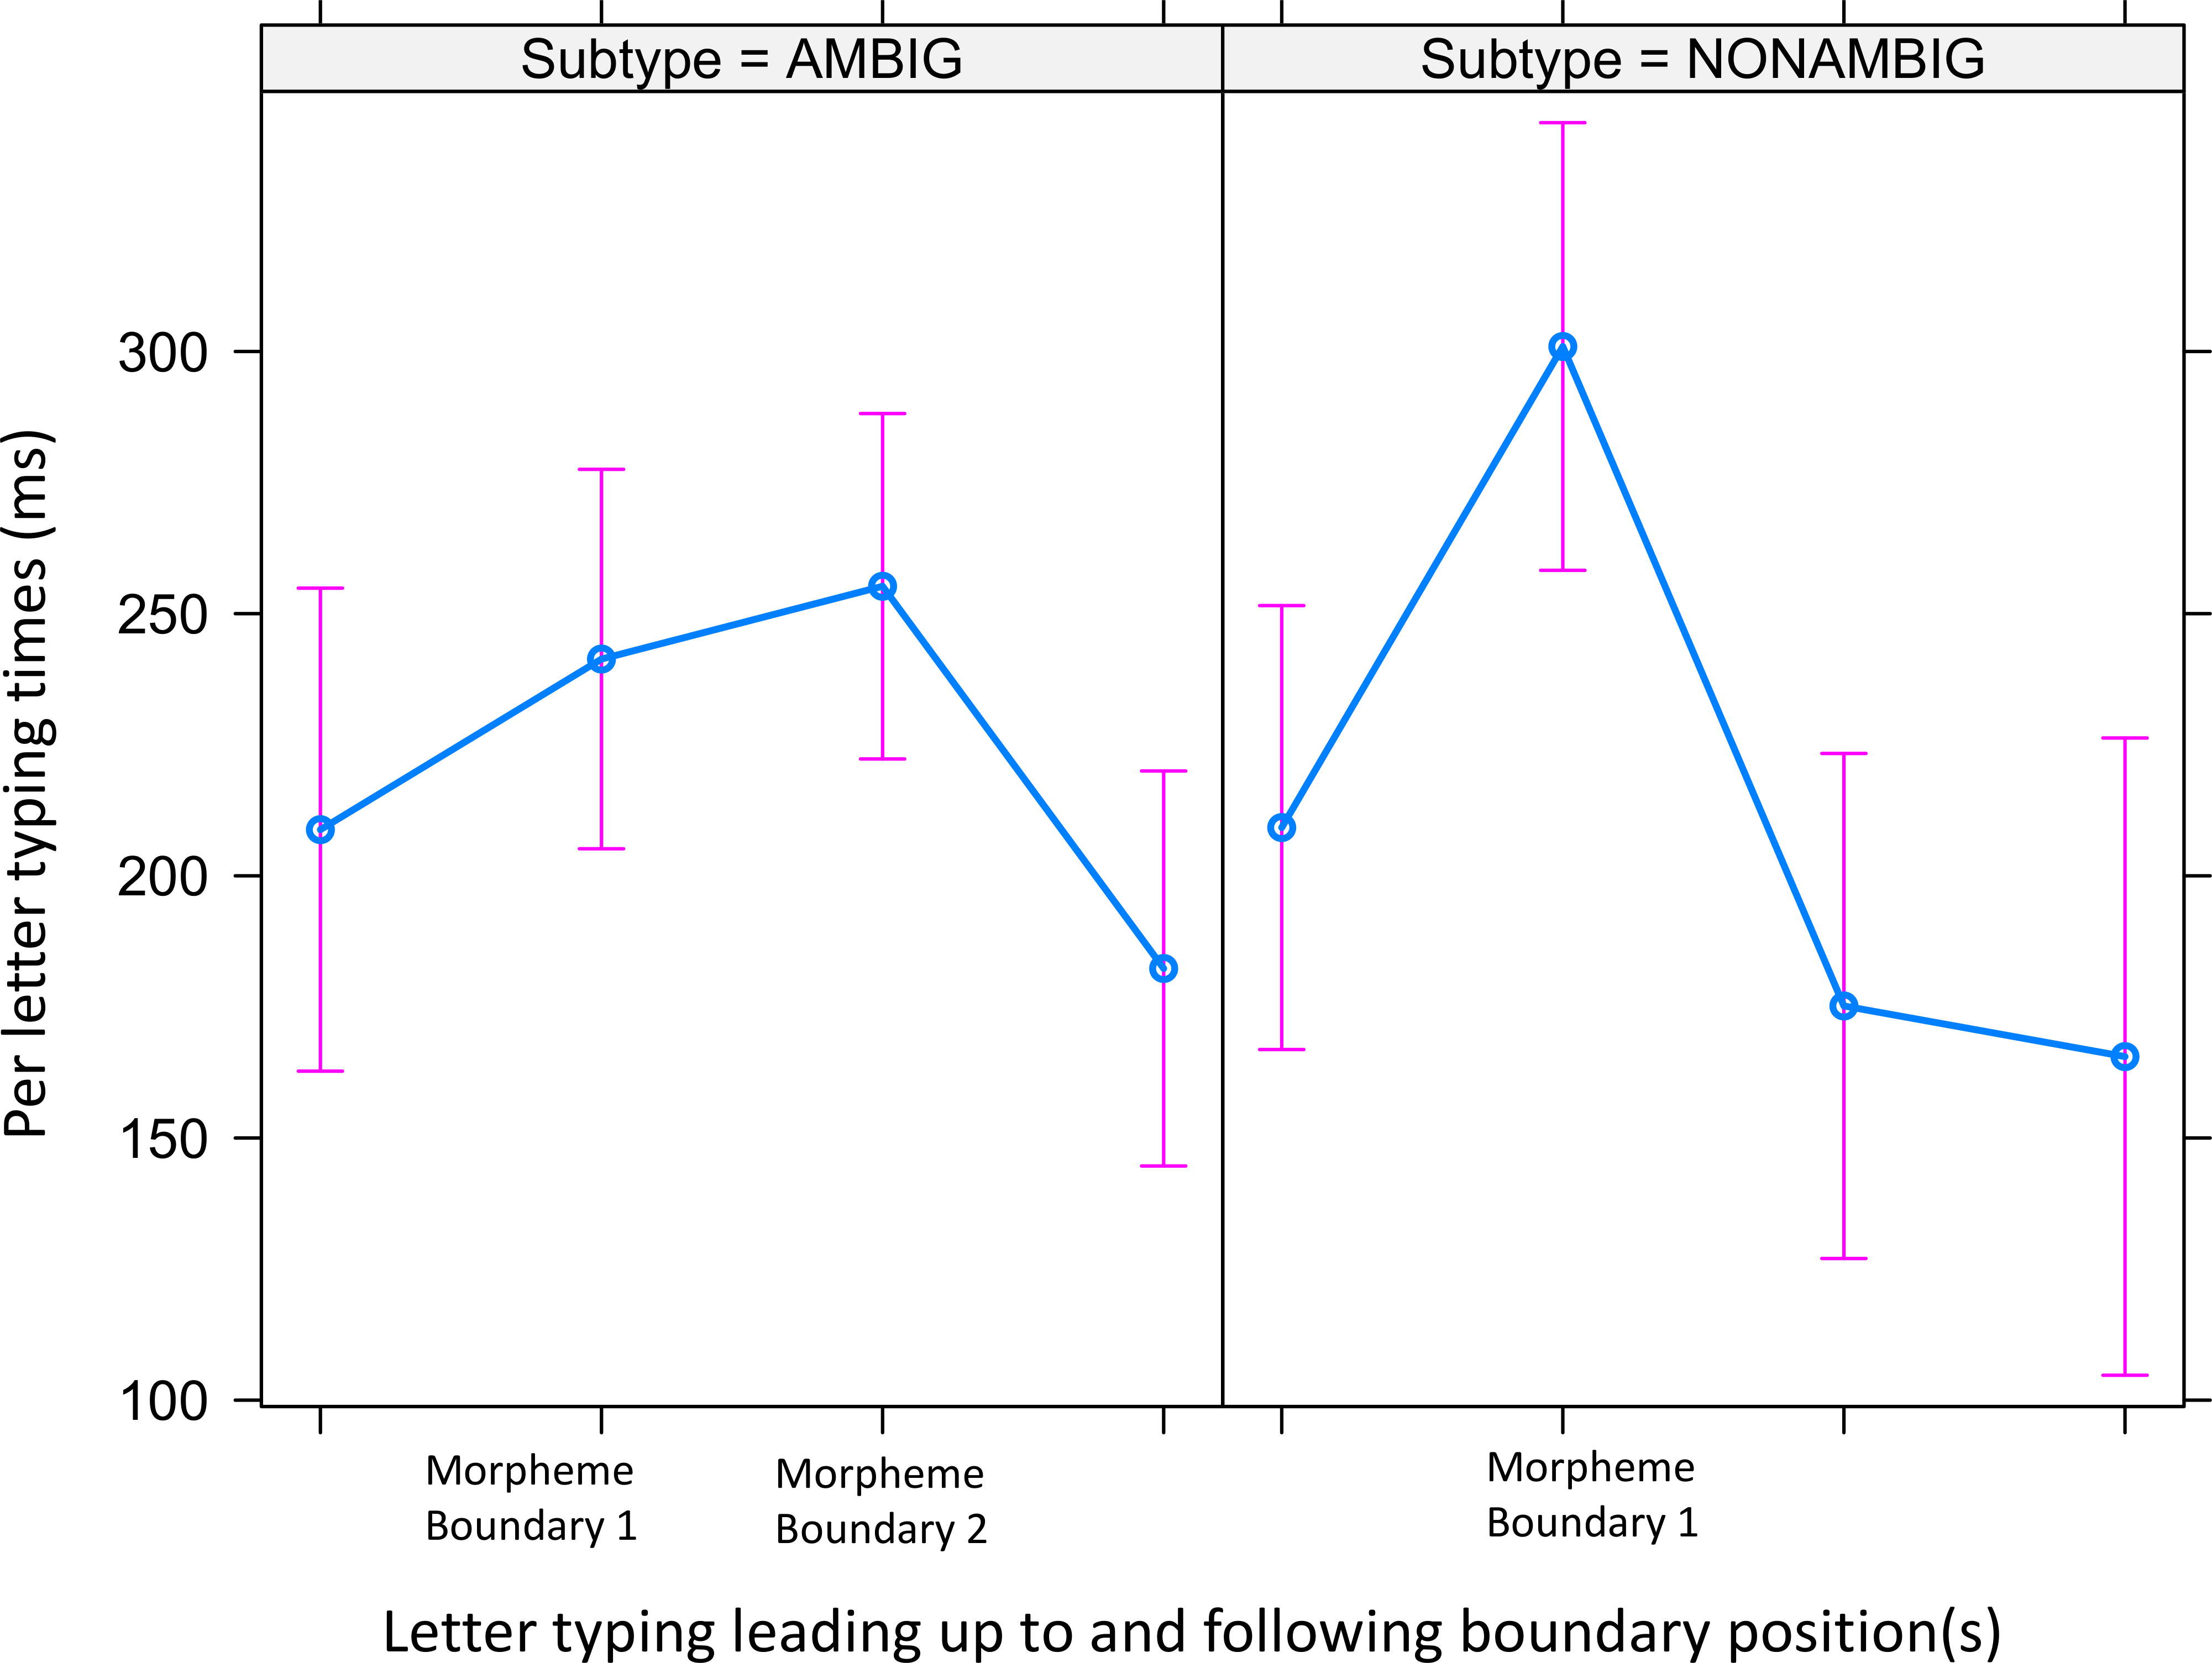
\includegraphics[width=.8\textwidth]{figures/Libbenfigure4.png}
\caption{\label{fig:libben:4}Per letter typing times for ambiguous novel compounds (e.g., \textit{clampeel}) and non-ambiguous novel compounds (e.g., \textit{anklecob}).}
\end{figure}

The notion of dual status accords with the view that lexical superstates characterize ambiguous strings such as \textit{clampeel}.  The data obtained through this experiment also seem to suggest that lexical superstates remain intact even when they could have been disambiguated as a result of reading aloud.  The data showed no interaction of response type (return key vs. reading aloud) with stimulus type (unambiguous vs. ambiguous with sound change vs. ambiguous without sound change).

\section{General discussion}\label{sec:libben:4}

This chapter has focused on English novel compounds as words that are themselves multiword expressions. I have claimed that the investigation of these structures can advance our understanding of morphological processing in general and the parsing of multiword lexical strings, in particular.  In that context, ambiguous novel compounds such as \textit{clampeel} may have a special role to play. Because they are ambiguous (e.g., can be parsed into \textit{clam-peel} or \textit{clamp-eel}) they enable us to investigate whether lexical processing results in the activation of one structure or all possible structures.  The prediction for these stimuli, in accordance with previous research by \citet{LibbenDerwingdeAlmeida1999}, was that we should see evidence of the activation of all potential constituents of ambiguous novel compounds in a word typing task.  This prediction is based on the claim that a core property of lexical representations is that they are shaped by patterns of lexical activity and they are commonly in a lexical superstate, rather than in any particular morphological configuration \citep{Libbeninpress}.  

An experiment was reported in which 24 participants each saw 45 novel compounds as progressively demasked stimuli and were required to type each of these as quickly and as accurately as possible. Typing times for each letter were recorded.

\subsection{Lexical superstates}\label{sec:libben:4.1}

The typing data are consistent with the lexical superstate hypothesis.  Whereas the non-ambiguous novel compounds such as \textit{anklecob} showed a sharp spike in letter typing times at the location between the two compound constituents, the ambiguous ones (e.g., \textit{clampeel}) showed more moderately elevated letter typing times at both putative inter-constituent locations (e.g., between \textit{clam} and \textit{peel} and between \textit{clamp} and \textit{eel}). This pattern of results is consistent with the view that such ambiguous words are in a lexical superstate so that the language user can employ the most appropriate interpretation of the string, depending on the situation.  I would argue that this phenomenon of lexical superstates is particularly easily seen in the case of ambiguous novel compounds but, in fact, is present in all putatively multimorphemic words. All such existing words are, by definition, structurally ambiguous. The simple reason for this is that they can at once have decomposed and undecomposed interpretations.  Again, lexical superstates allow the language user to employ whichever of these is most appropriate or most needed under particular circumstances.

An additional reason why the investigation of ambiguous novel compounds can be revealing of the underlying principles of lexical processing is that they constitute, by their nature, a controlled experiment.  They do not have existing whole word memory traces. So, when a participant encounters a novel compound, they must create an interpretation in real time. This interpretation can only be created with reference to possible internal constituents. Thus, these compounds provide us the controlled conditions under which we can investigate how lexical substrings are identified and how putative constituents are created.

\subsection{Action-based sublexical structure}\label{sec:libben:4.2}

If indeed, as I propose, morphological structure arises from lexical activity and words are more properly considered to be actions rather than things, an action-based account of how morphology comes about is required. I propose Fuzzy Forward Lexical Activation as such an account. Fuzzy Forward Lexical Activation has a maximally simple functional architecture. It claims that visual lexical processing in English proceeds from beginning to end and that, as soon as an initial lexical substring is identified, the system ``looks right'' to the end of the string for a possible concluding lexical substring.  It then continues in a left-to-right manner so that any possible initial substrings will be longer and any possible final substrings will be shorter. In this way, the heuristic only creates initial and final substrings (i.e., those that start at the beginning of the string and those that end at the end of the string, respectively).  All internal structures, therefore, will be binary.  Importantly, however, these binary structures will be overlapping for all multi-constituent strings.  These overlaps, created through lexical activity, constitute the structural lexical superstates for the words that are shown in \tabref{tab:libben:1}.

Thus, I claim that Fuzzy Forward Lexical Activation offers a simple mechanism for the activation of sublexical elements of a word. It renders hierarchical structure epiphenomenal, but at the same time offers an explanation for why English language users have multiple interpretation for ambiguous stimuli and left-branching and right-branching interpretations for words such as \textit{unlockable}.

\subsection{Action based lexical development is situation specific}\label{sec:libben:4.3}

It is important to note that the approach to sublexical structure discussed here is, by definition, linked to the specific experience that a language user has with language processing and the specific conditions under which language processing is taking place at the time of measurement.  Thus, for example, in this study, we did not observe a point at which overlaying alternative parses of ambiguous novel compounds are collapsed. It was expected that this might be observable by inspecting the interaction of response type (keypress vs. word naming) and type of ambiguous novel compounds (with sound change vs. without sound change). The reasoning behind this was that, in the word naming task, a choice between parsing alternatives would have to be made for stimuli such as \textit{babelarch}, which have different pronunciations, depending on the parsing choice.  The fact that this interaction was not observed may be related to the specific conditions of the experiment (e.g., the high density of ambiguous structures or perhaps the ability of participants to ``reset'' between the recognition and production components of each trial).

In addition to exploring the effects of varying task demands using stimuli of this sort, it would be valuable to investigate language demands.  It seems reasonable to expect that the “look-right to the end” feature of Fuzzy Forward Lexical Activation is developed as English language users adapt to the demands and opportunities created by the English writing system. It is very likely that this is a language-specific adaptation. For German, for example, it might be expected that language users might not create final substrings that must reach to the end of the word. The reason for this is that German has unspaced tri-constituent (and longer) compounds that the English writing system does not allow. Considerations such as these enhance the probability, in my view, that the conclusions we draw concerning language processing have enhanced ecological validity.  If we accept the view that words are patterns of action, rather than static representations, then we must also expect that their psycholinguistic instantiations will correspond with individual variability in language experience.

\section*{Acknowledgments}
The development of this chapter was supported by the Social Sciences and Humanities Research Council of Canada Partnership Grant 895-2016-1008 ``Words in the World''.

{\sloppy\printbibliography[heading=subbibliography,notkeyword=this]}
\end{document}
